\documentclass[11pt]{article}
\usepackage[top=2.54cm,bottom=2.54cm,left=1.27cm,right=1.27cm]{geometry}
\usepackage{graphicx}
\begin{document}
\title{Physics Behind the Simulation: A CS296 Report by Group 06}
\author{Sashank Gondala,\\
	120050050,\\
	\texttt{sgondala@cse.iitb.ac.in},\\
	Sundeep Routhu,\\
	120050048,\\
	\texttt{sundeep@cse.iitb.ac.in},\\
	Manik,\\
	120050006,\\
	\texttt{manik@cse.iitb.ac.in}}
\date{\today}
\maketitle
\pagebreak
\section{Introduction}
The purpose of this document is two-fold. 1st purpose is learning to use \LaTeX\ for writing reports.Other purpose is to show various additions incorporated in dominos.cpp. This document discusses the physics behind various new incorporations.  
\section{Physics behind the simulation}
\subsection{Collission between balls}
In this section, I describe the collission of two balls. As the external force on system of two balls is zero, Total linear momentum is conserved. Also, to find relation between initial and final velocities, we use equation of coefficient of restitution.\\
Equation of linear momentum is 
\begin{equation} m_{1}\bar{u_{1}}+m_{2}\bar{u_{2}}=m_{1}\bar{v_{1}}+m_{2}\bar{v_{2}}.\end{equation}\\
Equation of coefficient of restitution is\cite{irodov80}
\begin{equation}e=\frac{\bar{v_{2}}-\bar{v{1}}}{\bar{u_{1}}-\bar{u_{2}}}\end{equation}\\
Here $m_{1},m_{2}$ are Masses of ball 1 and 2;\\ $\bar{u_{1}},\bar{u_{2}}$ are Initial velocities of balls 1 and 2;\\
$\bar{v_{1}},\bar{v_{2}}$ are Final velocities of balls 1 and 2.\\
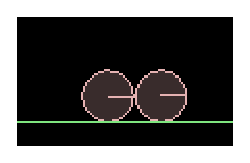
\includegraphics{2}
\subsection{Ball climbing the wedge}
In this section, I descibe the physics behind ball climbing up the incline plane. As net Force in horizontal direction is zero, Total energy of ball and wedge system is conserved.
 As wedge is fixed, Total energy of ball is conserved.\\Equation of conservation of energy is\cite{pandey08}
\begin{equation}\frac{1}{2}mu^{2}=mgh+\frac{1}{2}mv^{2}\end{equation}\\
 Here $m$ is mass of the ball,\\$g$ is acceleration due to gravity,\\$h$ is height of wedge,\\$u,v$ are initial and final velocities of ball.\\
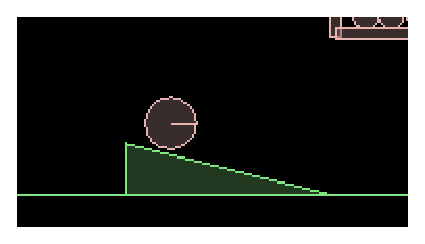
\includegraphics{1}  
\subsection{Ball rolling on semicircular platform}
These 3 equations combinely describe the motion of the ball\cite{verma06}. The first 2 represent translational motion of the ball\\
\begin{equation}N-mg\sin\theta=\frac{mv^{2}}{r}\end{equation}\\
\begin{equation}mg\cos\theta-f=ma\end{equation}\\
This equation represents the rotational motion of the ball\\
\begin{equation}fr=I\alpha\end{equation}\\
Here $m$ is mass of ball\\
$g$ is acceleration due to gravity\\
$f$ is friction\\
$r$ is radius of the ball\\
$v$ is speed of the ball\\
$N$ is normal reaction on the ball\\
$\theta$ is angle between vertical and tangential to point of contact\\
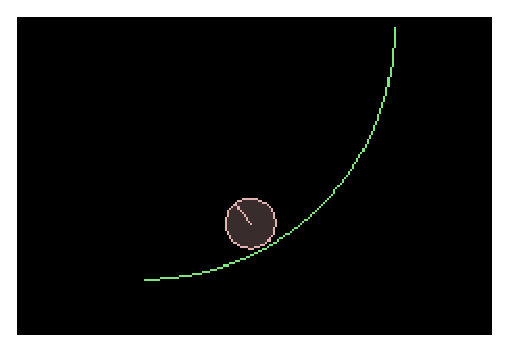
\includegraphics{3}
\section{Conclusion}
To formally conclude, This report has\\
\begin{itemize}
\item A section called 'Introduction' which describes the purpose of this report
\item A section called 'Physics behind the simulation' which describes new objects incorporated into base code and various physics laws governing them
\item Screenshots of newly added bodies
\item Conclusion
\end{itemize}
\bibliographystyle{plain}
\bibliography{references}
\end{document}
